\documentclass{article}
  %----------------------------------------------------------------------------------------
%	Author:	WangYifu
%	Create Date:	2017-02-14
%	Last Modify:	2018-09-01
%----------------------------------------------------------------------------------------
\usepackage[T1]{fontenc}
\usepackage{fourier}
\usepackage[english]{babel}
\usepackage{amsmath,amsfonts,amsthm}
\usepackage{geometry}
\usepackage{fancyhdr}
\usepackage{listings}
\usepackage{color}
\usepackage[yyyymmdd]{datetime}
\usepackage{graphicx}
\usepackage{float}
\usepackage{titling}
\usepackage{titlesec}
%-------------------------------%
%          Page Style           %
%-------------------------------%
\pagestyle{fancyplain}
\fancyhead{}
\fancyfoot[L]{}
\fancyfoot[C]{}
\fancyfoot[R]{\thepage}
\renewcommand{\headrulewidth}{0pt}
\renewcommand{\footrulewidth}{0pt}
\setlength{\headheight}{13.6pt}
\textwidth=6.5in
\textheight=9.0in
\headsep = 0.1in
\renewcommand{\baselinestretch}{1.2}
\geometry{a4paper,left=2cm,right=2cm,top=2cm,bottom=2cm}

%-------------------------------%
%           Font Size           %
%-------------------------------%
\newcommand{\erhao}{\fontsize{22.1pt}{\baselineskip}\selectfont}
\newcommand{\sanhao}{\fontsize{16.1pt}{\baselineskip}\selectfont}
\newcommand{\sihao}{\fontsize{14.1pt}{\baselineskip}\selectfont}
\newcommand{\xiaosi}{\fontsize{12.1pt}{\baselineskip}\selectfont}
\newcommand{\wuhao}{\fontsize{10.5pt}{\baselineskip}\selectfont}
\newcommand{\setFontSize}[1]{\fontsize{#1}{\baselineskip}\selectfont}
\titleformat{\section}{\sanhao\bfseries}{$\bullet$}{5pt}{}

%-------------------------------%
%             Title             %
%-------------------------------%
\newcommand{\horrule}[1]{\rule{\linewidth}{#1}}
\renewcommand{\dateseparator}{ - }
\def\Assignment{Assignment Title}
\title{
\vspace{-2cm}
\normalfont \normalsize
\textsc{Washington University in St. Louis} \\ [0pt]
\horrule{1pt} \\[0.4cm]
\huge {\bf\Assignment}
}
\author{467261 - Yifu Wang}
\date{\normalsize\today\\\horrule{1pt} \\[0.5cm]}

%-------------------------------%
%           TableList           %
%-------------------------------%
\newcommand{\deflabel}[1]{#1\hfill}
\newenvironment{tlist}[1]{
	\begin{list}{}{
			\settowidth{\labelwidth}{\bf#1}
			\setlength{\leftmargin}{\labelwidth}
			\addtolength{\leftmargin}{\labelsep}
			\renewcommand{\makelabel}{\bf\deflabel}}}{
	\end{list}
}

%-------------------------------%
%             Code              %
%-------------------------------%
\definecolor{gray}{RGB}{191,191,191}
\definecolor{dkgreen}{RGB}{96,139,78}
\definecolor{mauve}{RGB}{206,145,120}

\lstset{ %
	language=C++,                % the language of the code
	% basicstyle=\textheight,           % the size of the fonts that are used for the code
	numbers=left,                   % where to put the line-numbers
	numberstyle=\color{black},  % the style that is used for the line-numbers
	stepnumber=0,                   % the step between two line-numbers. If it's 1, each line 
	% will be numbered
	numbersep=5pt,                  % how far the line-numbers are from the code
	backgroundcolor=\color{gray},      % choose the background color. You must add \usepackage{color}
	showspaces=false,               % show spaces adding particular underscores
	showstringspaces=false,         % underline spaces within strings
	showtabs=false,                 % show tabs within strings adding particular underscores
	frame=false,                   % adds a frame around the code
	rulecolor=\color{gray},        % if not set, the frame-color may be changed on line-breaks within not-black text (e.g. commens (green here))
	tabsize=2,                      % sets default tabsize to 2 spaces
	captionpos=b,                   % sets the caption-position to bottom
	breaklines=true,                % sets automatic line breaking
	breakatwhitespace=false,        % sets if automatic breaks should only happen at whitespace
	keywordstyle=\color{blue},          % keyword style
	commentstyle=\color{dkgreen},       % comment style
	stringstyle=\color{mauve},         % string literal style
}

  \def\Assignment{CES571S - Spectre - Final Report}
\begin{document}
\maketitle
\section{Introduction}
Spectre is a vulnerability that affects modern microprocessors that perform branch prediction. On most processors, the speculative execution resulting from a branch misprediction may leave observable side effects that may reveal private data to attackers. For example, if the pattern of memory accesses performed by such speculative execution depends on private data, the resulting state of the data cache constitutes a side channel through which an attacker may be able to extract information about the private data using a timing attack.
\newline
\newline
Spectre attack can be conduct on browser victims. But this require attacker to send an attacker controled code to victims and execute it localy. Furthermore this attack can only retrieve the data from the process which runing the attacker controled code due to the seperation policy defined by mordern browser.
\newline
\newline
Howerver a derivation of spectre attack, netspectre, a generic remote Spectre
variant 1 attack, could allow attackers to read arbitrary memory from the systems available on the network containing the required Spectre gadgets—a code that performs operations like reading through an array in a loop with bounds check on each iteration.
\newline
\newline
The original goal of this project is to setup a spectre attack cross processes, which now I knew impractical. So instead I implement a PoC of netspectre attack.
\newline
\newline
The project repository is held by this \href{https://github.com/Luna1996/WUSTL/tree/master/571/Project}{link}.

\section{Implement local attack}
The local attack is fairly easy to implement. By using C/C++, you can directly execute assmembly language in your program, which allow to clear cache and measure system ticks manually, both of which are very importent for a successful spectre attack.
\newline
\newline
This program got auto-deleted all the time unless I turn off real time virus detection. But it still won't upload to github. So I compressed it. Basicly this program will retreive a build-in string array's value. Most of it was done by following the guide of SEED lab. But when runing on my machine. Some code will be optimized out sometimes. Those code is commened in source.
\begin{figure}[H]\centering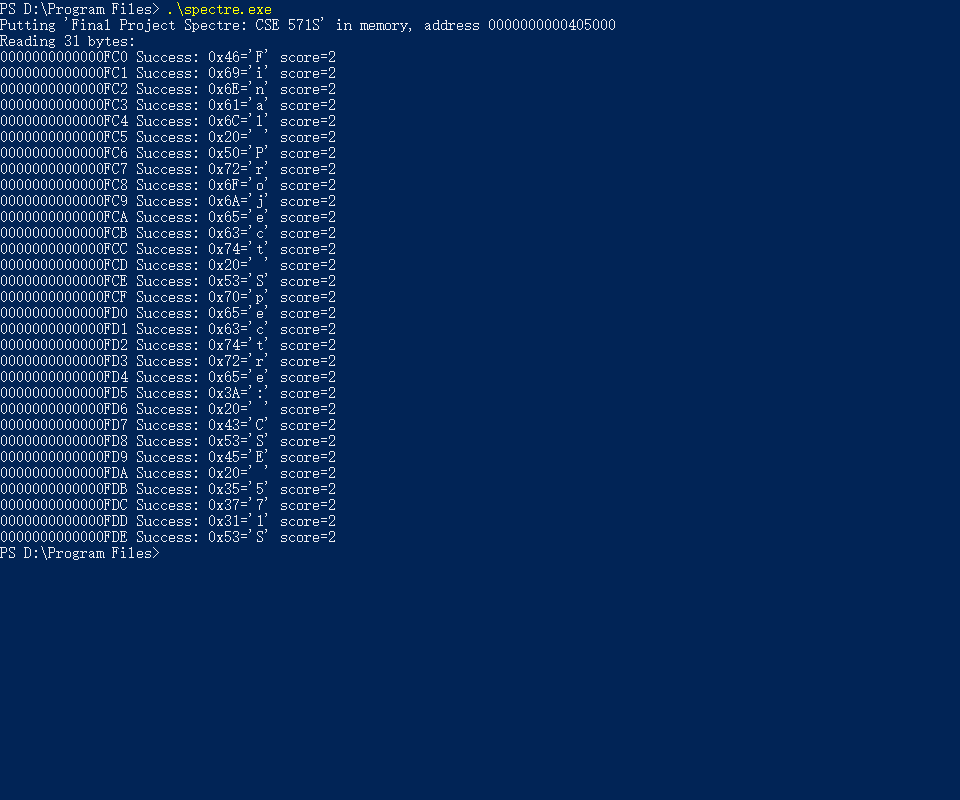
\includegraphics[width=\textwidth]{01.png}\end{figure}
\section{Implement browser attack}
Since JavaScript couldn't manually control the caches. We have to evict cache before every iteration using some unrelavent junk data block. And since chrome has already patched this vulnerability by disabled SharedArray default. You need to enable it from setting and then you maight want to check if your browser is vulnerabel to spectre by \href{https://xlab.tencent.com/special/spectre/spectre_check.html}{this site}.
\newline
\newline
This site will retreive a build-in SharedArray data. But unlike local attack. Browser attack will sometimes be inaccurate due to the timer, and cache eviction. This is done by following the discreption in paper [1].
\begin{figure}[H]\centering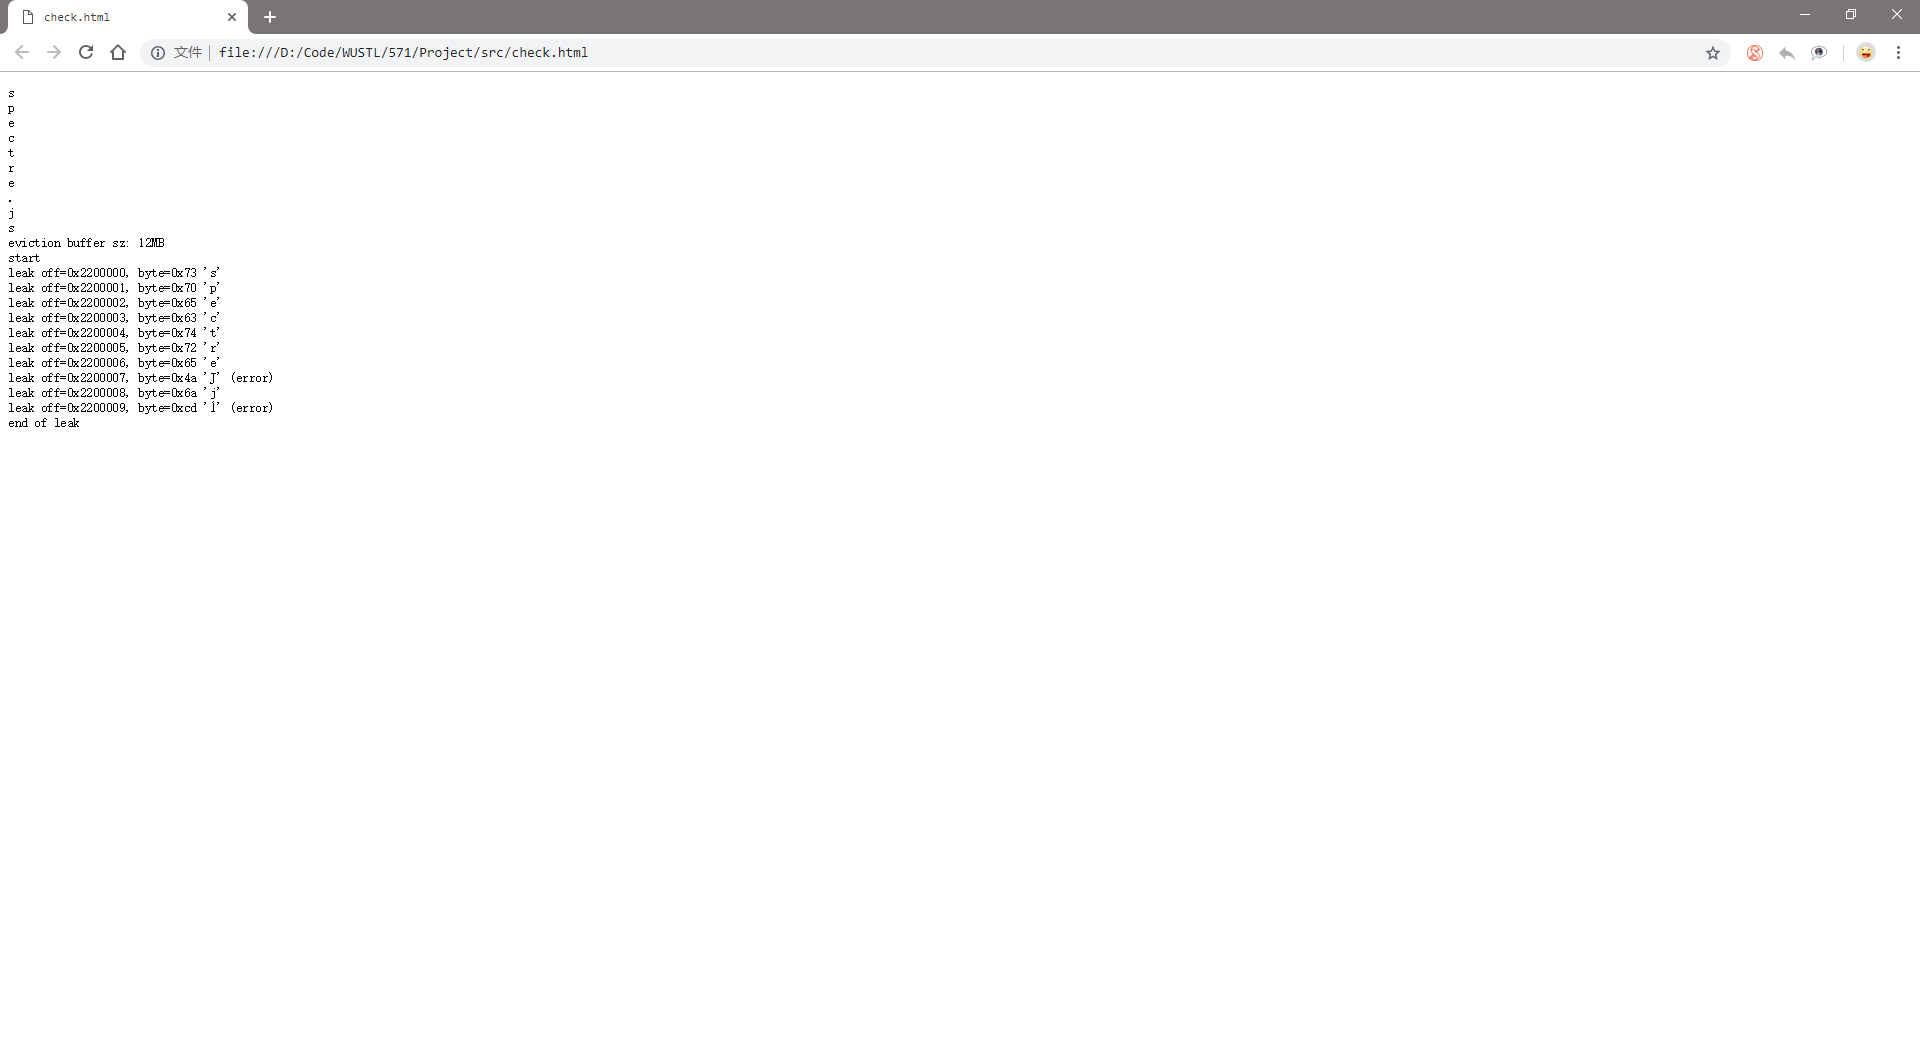
\includegraphics[width=\textwidth]{02.png}\end{figure}
\section{Implement netspectre attack}
Basicly to complete a netspectre attack you need so call 'gadget' be pre-insert into user's machine. Which will listen to attacker's remote packet to mistraining the predictor and send back the bits value. Meanwhile the attacker side will measure the response timing and repeat this process as many as possible until the result is satisfide.
\newline
\newline
To get this attack work, firstly you should open netspectre.html and set up a single byte data. Then open NetSpectre.exe and set the victim ip, this program designed to be run in the attacker's machine, but victim and attacker should under the same subnet. By clicking the start button, the program should start to measure the response time for each bit. It's might take more than one hour to retreive one byte from netspectre.html.
\begin{figure}[H]\centering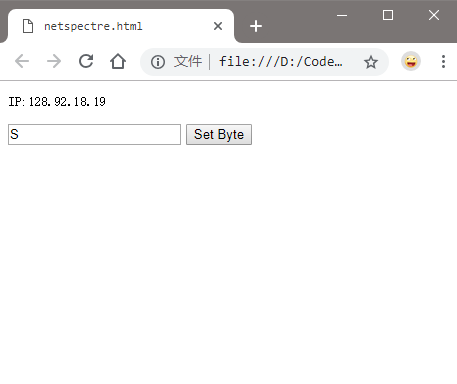
\includegraphics{05.png}\end{figure}
\begin{figure}[H]\centering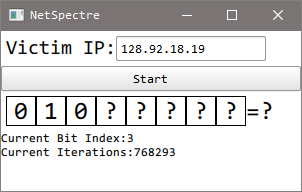
\includegraphics{03.png}\end{figure}
\begin{figure}[H]\centering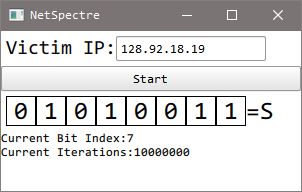
\includegraphics{04.png}\end{figure}
\section{Conclution}
At present, spectre or netspectre is not a very serious problem that will endanger most common user. Since both of them need to pre-send some attacker code into user's machine. And even though netspectre attack claims to be able to retreive any data from a machine, but it's extremely slow. It's only reveal 15 bits per hour, namely 1 GB per 60822 years.
\section{Reference}
[1]:\href{https://spectreattack.com/spectre.pdf}{Spectre}
\newline
[2]:\href{https://arxiv.org/pdf/1807.10535.pdf}{NetSpectre}
\end{document}